Los asistentes de demostración son herramientas que facilitan la escritura y chequeo de demostraciones en una computadora. Pueden ser usados para formalizar teoremas, realizar verificación formal de programas, entre otros. A diferencia de escribir demostraciones y chequearlas manualmente, el uso de asistentes permite la colaboración a gran escala: no es necesario confiar ni revisar a detalle las demostraciones que hace el resto del equipo, alcanza con que el asistente las considere válidas. También facilitan el proceso de generar demostraciones mediante LLMs, que muchas veces generan razonamientos lógicos erróneos, lo cual sería inviable chequear a mano. Pero podemos delegar su verificación al asistente.

Trabajan con distintas \textit{teorías}. Por ejemplo, el asistente Mizar con lógica de primer orden, Coq con teoría de tipos (cálculo de construcciones o CoC) y Agda también (teoría unificada de tipos dependientes, basada en teoría de tipos de Martin-Löf).

Una propiedad deseable cumplida por muchos asistentes es el \textbf{criterio de De Bruijn}. En principio, para estar seguros de que una demostración es correcta sería necesario confiar en la implementación del asistente, que puede ser muy compleja. Un asistente se dice que cumple con el criterio si construye una demostración en un formato elemental, sencillo, que pueda ser chequeada por un programa independiente, escrito por cualquiera que desconfíe de la implementación original del asistente. De esa forma no es necesario confiar en ella.

En este trabajo implementamos una asistente de demostración \textit{PPA}
(\textit{Pani's proof assistant}) inspirado en Mizar. Trabaja sobre teorías de
lógica clásica de primer orden. Cumple con el criterio de De Bruijn porque
\textit{certifica} las demostraciones en el lenguaje de alto nivel \ppaLang{},
generando demostraciones de bajo nivel de deducción natural: un sistema lógico
que permite escribir demostraciones mediante reglas de inferencia. Además,
implementa extracción de testigos de existenciales. Su sintaxis está inspirada
en el \textit{mathematical vernacular} introducido por Freek Wiedijk en
\cite{freek-mv}, que tiene por objetivo ser lo más parecido posible al lenguaje
natural. No es un demostrador automático de teoremas, pero incluye un pequeño
demostrador heurístico para lógica de primer orden y completo para
proposicional, que simplifica la escritura de demostraciones.

Para la extracción de testigos, es deseable que las demostraciones sean
\textbf{constructivas}: una demostración de $\exists \var . \pred(\var)$ nos
debe decir cómo encontrar a un objeto $\term$ que cumpla con $\pred(\term)$. PPA
usa lógica clásica, que no siempre es constructiva por los principios de
razonamiento clásicos como LEM. Siempre vale $\form \fOr \fNot
\form$, y podemos demostrar usando eso sin determinar exactamente cual de las
dos vale. Los asistentes como Coq lo aseguran mediante el uso de \textbf{lógica
intuicionista}, que siempre es constructiva.

En este trabajo, la extracción se hace de forma \textit{indirecta} en dos pasos.
Primero hacemos uso de la \textbf{traducción de Friedman}
\cite{miquel-friedman}, que permite traducir una demostración clásica a una
intuicionista para cierta clase de fórmulas: las $\classPiTwo$, de la pinta
$\forall \var_1 \dots \forall \var_n . \exists \varTwo . \anyForm$. Luego,
\textit{normalizamos} la demostración intuicionista, y de su forma normal
extraemos el testigo del existencial. No conocemos un asistente de demostración
de lógica clásica que implemente la traducción de Friedman original para extraer
testigos. La implementación de un mecanismo de extracción indirecto es el aporte principal de este trabajo.

\section{Lógica de primer orden}

A continuación se presentan definiciones preliminares de lógica de primer orden. Suponemos dados,

\begin{itemize}
    \item Un conjunto infinito numerable de \textbf{variables}
    \(
        \{\var, \varTwo, \varThree, \dots\}
    \)
    \item Un conjunto infinito numerable de \textbf{símbolos de función}
    \(
        \{\fun, \funTwo, \funThree, \dots\}
    \)
    \item Un conjunto infinito numerable de \textbf{símbolos de predicado}
    \(
        \{\pred, \predTwo, \predThree, \dots\}
    \)
\end{itemize}

\begin{definition}[Términos]
    Los términos están dados por la gramática
    \begin{align*}
        \term ::= &\ \var                               &\text{(variables)} \\
                  & \mid \fun(\term_1, \dots, \term_n) &\text{(funciones)}
    \end{align*}
\end{definition}

\begin{definition}[Fórmulas]
    Las fórmulas están dadas por la gramática
    \begin{align*}
        \form, \formTwo ::=
         & \ \pred(\term_1, \dots, \term_n) & (\text{predicados})                \\
         & \mid \fFalse \mid \fTrue             & \text{(verdadero y falso)}         \\
         & \mid \form \fAnd \formTwo        & \text{(conjunción)}                \\
         & \mid \form \fOr \formTwo         & \text{(disyunción)}                \\
         & \mid \form \fImp \formTwo        & \text{(implicación)}               \\
         & \mid \fNot \form                 & \text{(negación)}                  \\
         & \mid \forall \var . \form        & \text{(cuantificador universal)}   \\
         & \mid \exists \var . \form        & \text{(cuantificador existencial)}
    \end{align*}

    Los predicados son \textbf{fórmulas atómicas}. Los de aridad 0 además son llamados \textit{variables proposicionales}.
\end{definition}

\begin{notation*}
    Usamos
    \begin{itemize}
        \item $\formLit, \formLitTwo, \formLitThree, \dots$, $\form, \formTwo, \formThree, \dots$ y $\anyForm, \anyFormTwo, \dots$ para referirnos a fórmulas.
        \item $\term, \termTwo, \dots$ para referirnos a términos
    \end{itemize}
\end{notation*}

\begin{definition}[Variables libres y ligadas]
    Las variables pueden ocurrir libres o ligadas. Los cuantificadores ligan a
    las variables, y usamos $\fv(\form)$ para referirnos a las variables libres
    de una fórmula. Se define por inducción estructural de la siguiente forma.

    \begin{itemize}
        \item Términos
        \begin{align*}
            \fv{\var} &= \{ \var \}\\
            \fv{\fun(\term_1, \dots, \term_n)} &= \bigcup_{i \in 1\dots n} \fv{t_i} 
        \end{align*}
    
        \item Fórmulas
        \begin{align*}
            \fv{\fFalse} &=\emptyset\\
            \fv{\fTrue} &=\emptyset \\
            \fv{\pred(\term_1, \dots, \term_n)} &= \bigcup_{i \in 1\dots n} \fv{t_i} \\
            \fv{\form \fAnd \formTwo} &= \fv{\form} \cup \fv{\formTwo}\\
            \fv{\form \fOr \formTwo} &=\fv{\form} \cup \fv{\formTwo}\\
            \fv{\form \fImp \formTwo} &=\fv{\form} \cup \fv{\formTwo}\\
            \fv{\fNot \form} &=\fv{\form}\\
            \fv{\forall \var . \form} &= \fv{\form} \setminus \var \\
            \fv{\exists \var . \form} &= \fv{\form} \setminus \var
        \end{align*}
    \end{itemize}
\end{definition}


\section{Arquitectura de \ppaTool{}}

A lo largo del trabajo, usaremos ``PPA'' para referirnos a dos cosas separadas: \ppaLang{} el lenguaje para escribir demostraciones, y \ppaTool{} la herramienta que implementa el lenguaje y con su extracción de testigos. Esta última está implementada en \textbf{Haskell}. Funcionalmente tiene la siguiente arquitectura, representada en la \fullref{intro:fig:ppa-arch}

\begin{itemize}
    \item El usuario escribe una demostración en alto nivel en el lenguaje \ppaLang{}
    \item Puede \textit{chequear} la demostración, que primero la \textbf{certifica} generando una demostración de deducción natural (el ``certificado'') que es chequeada por su correctitud.
    \item Luego, si es una demostración de un existencial, el usuario puede optar por \textit{extraer un testigo}: primero se \textbf{traduce} la demostración de clásica a intuicionista, y luego se reduce hacia su formal normal de la cual se puede tomar el testigo.
\end{itemize}

Las definiciones principales son las siguientes

\begin{itemize}
    \item El tipo \mintinline{haskell}{type Result a = Either String a} es la mónada principal que se usa para permitir devolver resultados correctos o errores.
    \item \mintinline{haskell}{certify :: Program -> Result Context}. Implementada por el módulo \texttt{PPA.Certifier}. Certifica un \textit{programa} (axiomas y teoremas) generando un \textit{contexto} (una demostración en deducción natural para cada teorema).
    \item \mintinline{haskell}{check :: Env -> Proof -> Form -> CheckResult}.
    Implementada por el módulo \texttt{ND.Checker}. Chequea una demostración de una fórmula asumiendo un entorno o contexto de demostración.
    \item \mintinline{haskell}{translateFriedman :: Proof -> FormPi02 -> (Proof, R)}. Implementada por el módulo \texttt{Extractor.Translator.Proof}. Traduce una demostración clásica de una fórmula $\classPiTwo$ generando una demostración intuicionista, usando la traducción de Friedman relativizando la negación con \mintinline{haskell}{R}.
    \item \mintinline{haskell}{reduce :: Proof -> Proof}. Reduce una demostración a su forma normal. Implementada en el módulo \texttt{Extractor.Reducer}.
\end{itemize}

\begin{figure}[h]
    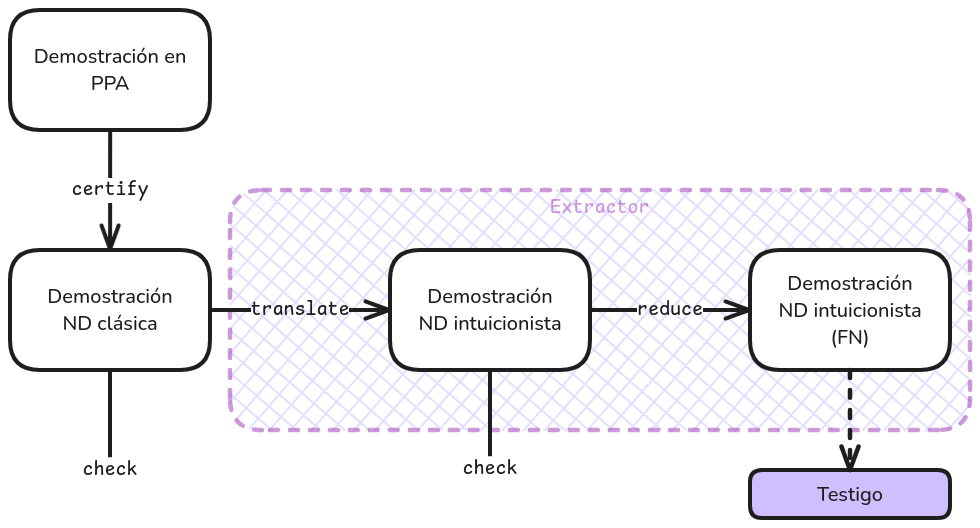
\includegraphics[scale=0.42]{img/arch.png}
    \centering
    \caption{Arquitectura funcional de \ppaTool{}}
    \label{intro:fig:ppa-arch}
\end{figure}

\section{Estructura del escrito}

El trabajo se divide en 5 capítulos principales además de la introducción y la conclusión. Comenzamos por el \fullref{chap:nd} en el que se presenta de forma completa el sistema de deducción natural usado para los certificados. Se introducen las reglas de inferencia junto con sus intuiciones, el concepto de \textit{reglas admisibles}, demostraciones de ejemplo y algunos algoritmos implementados: chequeo (función \mintinline{haskell}{check}), alfa equivalencia de fórmulas y sustitución sin capturas.

En el \fullref{chap:ppa} introducimos el lenguaje desde el punto de vista de un usuario: cómo están compuestos los programas, cómo usar el pequeño demostrador (\lstinline{by}) para facilitar la escritura de demostraciones, y una descripción exhaustiva de todos los comandos soportados. En \fullref{chap:ppa-certifier} se muestra la implementación interna del \textit{certificador} de PPA, cómo se generan demostraciones en deducción natural a partir de programas (la función \mintinline{haskell}{certify}). De forma central se explica el funcionamiento del \lstinline{by}, que es el corazón del certificador.

En el \fullref{chap:witness-extraction} se muestra el proceso completo de extracción de testigos, comenzando por la traducción de Friedman y luego la normalización de demostraciones intuicionistas (\mintinline{haskell}{translateFriedman} y \mintinline{haskell}{reduce}).

Finalmente, en el \fullref{chap:ppa-tool} se detallan los pasos para instalar y usar la herramienta \ppaTool{}, y se mencionan algunos detalles de implementación como la arquitectura del programa a nivel módulos y dependencias entre ellos, el compilador y el modelado de deducción natural.